%\documentclass[10pt,notes]{beamer}       % print frame + notes
%\documentclass[10pt, notes=only]{beamer}   % only notes
\documentclass[11pt]{beamer}              % only frames

%%%%%% IF YOU WOULD LIKE TO CREATE LECTURE NOTES COMMENT OUT THE FOlLOWING TWO LINES
%\usepackage{pgfpages}
%\setbeameroption{show notes on second screen=bottom} % Both

\usepackage{graphicx}
\DeclareGraphicsExtensions{.pdf,.png,.jpg}
\usepackage{color}
\usetheme{winslab}
\usepackage[utf8]{inputenc}
\usepackage[english]{babel}
\usepackage{amsmath}
\usepackage{amsfonts}
\usepackage{amssymb}




\usepackage{algorithm2e,algorithmicx,algpseudocode}
\algnewcommand\Input{\item[\textbf{Input:}]}%
\algnewcommand\Output{\item[\textbf{Output:}]}%
\newcommand\tab[1][1cm]{\hspace*{#1}}

\algnewcommand{\Implement}[2]{\item[\textbf{Implements:}] #1 \textbf{Instance}: #2}%
\algnewcommand{\Use}[2]{\item[\textbf{Uses:}] #1 \textbf{Instance}: #2}%
\algnewcommand{\Trigger}[1]{\Statex{\textbf{Trigger:} (#1)}}%
\algnewcommand{\Events}[1]{\item[\textbf{Events:}] #1}%
\algnewcommand{\Need}[1]{\item[\textbf{Needs:}] #1}%
\algnewcommand{\Event}[2]{\Statex \item[\textbf{On#1:}](#2) \textbf{do}}%
\algnewcommand{\Trig}[3]{\State \textbf{Trigger}  #1.#2 (#3) }%
\def\true{\textbf{T}}
\def\false{\textbf{F}}


\author[Ersel Hengirmen]{Ersel Hengirmen\\\href{mailto:ehengirmen@hotmail.com}{ehengirmen@hotmail.com}}
%\author[J.\,Doe \& J.\,Doe]
%{%
%  \texorpdfstring{
%    \begin{columns}%[onlytextwidth]
%      \column{.45\linewidth}
%      \centering
%      John Doe\\
%      \href{mailto:john@example.com}{john@example.com}
%      \column{.45\linewidth}
%      \centering
%      Jane Doe\\
%      \href{mailto:jane.doe@example.com}{jane.doe@example.com}
%    \end{columns}
%  }
%  {John Doe \& Jane Doe}
%}

\title[WINS Beamer Template]{AWERBUCH’S SYNCHRONIZERS (ALPHA, BETA, GAMMA)}
%\date{} 

\begin{document}
	
\begin{frame}[plain]
\titlepage
\note{In this talk, I will present .... Please answer the following questions:
\begin{enumerate}
\item Why are you giving presentation?
\item What is your desired outcome?
\item What does the audience already know  about your topic?
\item What are their interests?
\item What are key points?
\end{enumerate}
}
\end{frame}

\begin{frame}[label=toc]
    \frametitle{Outline of the Presentation}
    \tableofcontents[subsubsectionstyle=hide]
\note{ The possible outline of a talk can be as follows.
\begin{enumerate}
\item Outline 
\item Problem and background
\item Design and methods
\item Major findings
\item Conclusion and recommendations 
\end{enumerate} Please select meaningful section headings that represent the content rather than generic terms such as ``the problem''. Employ top-down structure: from general to more specific.
}
\end{frame}
%
%\part{This the First Part of the Presentation}
%\begin{frame}
%        \partpage
%\end{frame}
%
\section{The Problem}
%\begin{frame}
%        \sectionpage
%\end{frame}

\begin{frame}{The problem}
	\begin{block}{Synchronization} 
		Synchronization in distributed systems is crucial for maintaining coherence and ensuring consistent behavior across processes, especially in transitioning from synchronous to asynchronous environments. 
	\end{block}
	\note{}
\end{frame}

\section{The Contribution}
\begin{frame}
	\frametitle{What is the solution/contribution}
	\framesubtitle{}
	\begin{itemize}
		\item Implementation of Alpha, Beta, Gamma Algorithms on the AHCv2 platform.
		\item Anlysis of the algorithms within different topologies
	\end{itemize}
\end{frame}


\section{Motivation/Importance}
\begin{frame}
	\frametitle{Motivation/Importance-1}
	These synchronizers play a pivotal role in distributed systems by enabling coordination and consistency among processes operating in asynchronous environments. Their importance lies in their ability to bridge the gap between synchronous and asynchronous systems, allowing distributed applications to maintain coherence and achieve desired outcomes despite the lack of a global clock or fixed time intervals.
\end{frame}

\begin{frame}
	\frametitle{Motivation/Importance-2}
	Without effective synchronizers, distributed systems would struggle to ensure consistent behavior, leading to potential issues such as data inconsistencies, race conditions, and overall system instability. Therefore, these synchronizers serve as fundamental building blocks for the reliable and efficient operation of distributed systems in various domains, including cloud computing, networking, and parallel computing.
\end{frame}

\section{Background/Model/Definitions/Previous Works}


\subsection{Model, Definitions}

\frame{
	\frametitle{Model, Definitions}
	\begin{itemize}
		\item Synchronization: The process of coordinating actions or events across distributed entities to maintain coherence and consistency.
		\item Asynchronous Systems: Distributed systems where processes operate independently without a global clock or fixed time intervals.
	\end{itemize} 
	Background and this slide can be combined....
}

\subsection{Background, Previous Works}
\begin{frame}{Background}
	The 1985 paper Awerbuch "Complexity of network synchronization" proposes the method for alpha beta gamma synchronizers(without naming them as alpha beta gamma) and analyzes the trade-offs between them in this paper. So in essence its a paper that introduces simple methodologies for designing efficient distributed algorithms in asynchronous networks.
	
\end{frame}




\section{Contribution}

\begin{frame}
	\frametitle{Alpha}
	
	\begin{itemize}
		\item In the alpha synchronizer, every node sends a message to every neighbor in every round(so that neighboor can synchronize with it)
		\begin{itemize}
			\item If no message needs to be sent to that neighboor, node sends a dummy message to that neighboor.
		\end{itemize}
		\item The receiver waits until it receives a message from every neighbor for a particular round before proceeding to the next round.
	\end{itemize}
	
\end{frame}

\begin{frame}
	\frametitle{Alpha Algorithm}
	
	\begin{center}
		\begin{figure}
			\centering
			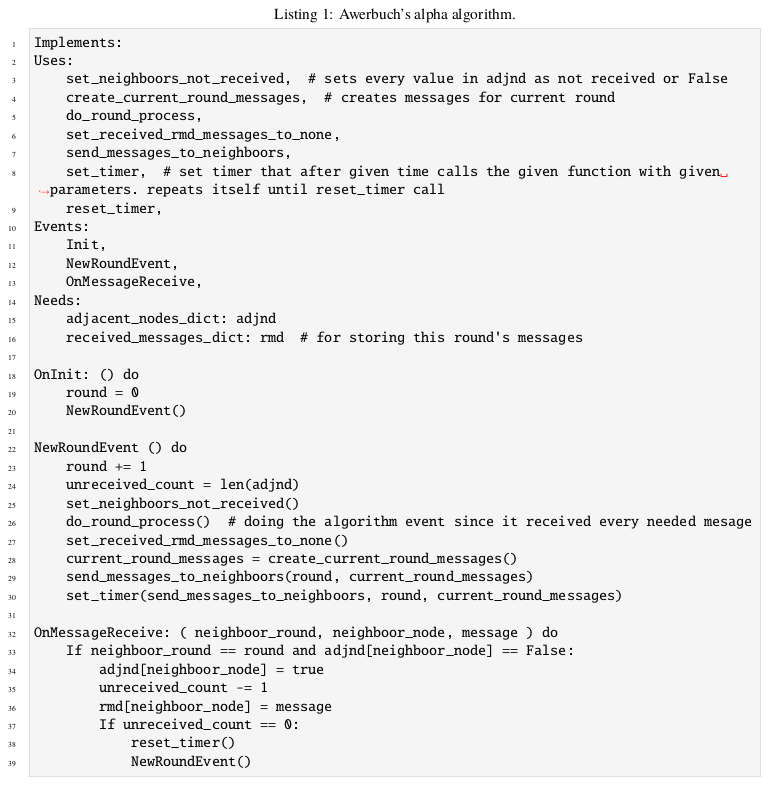
\includegraphics[scale=0.2]{figures/alpha.png}
		\end{figure}
	\end{center}
	
\end{frame}

\begin{frame}
	\frametitle{Beta}
	\begin{itemize}
		\item In the beta synchronizer, messages sent by processes are acknowledged by their receivers.
		\item Senders wait until they receive acknowledgments (ACKs) from all receivers for the messages they sent in a particular round.
		\begin{itemize}
			\item That is why since its a reliable connection we act like receive happens only ones(think of TCP)
		\end{itemize}
		\item Once all ACKs are received and all OKs from child nodes are received, the node sends ok to parent node.
		\item Once root receives OK from its parent nodes it broadcasts GO signifying the start of new round
	\end{itemize}
\end{frame}

\begin{frame}
	\frametitle{Beta Algorithm}
	
	\begin{center}
		\begin{figure}
			\centering
			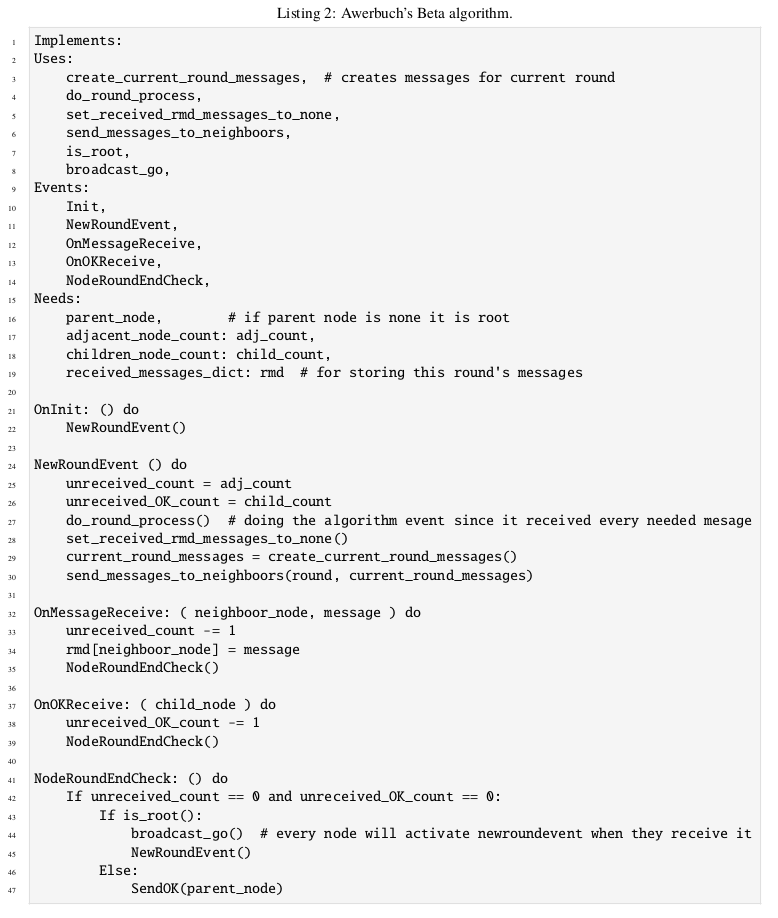
\includegraphics[scale=0.2]{figures/beta.png}
			\caption{}
			\label{fig:awesome_image}
		\end{figure}
	\end{center}
	
\end{frame}



\begin{frame}
	\frametitle{Gamma}
	\begin{itemize}
		\item The gamma synchronizer is the merge of both alpha and beta synchronizers. It does this by having multiple roots which all have their own spanning trees where:
		\begin{itemize}
			\item The beta algorithm runs within each tree 
			\item The alpha algorithm runs between trees
		\end{itemize}
		\item In here in addition to beta when the root of a tree gets all acks and OKs, it sends ready to the roots of all adjacent trees (and itself).
		\begin{itemize}
			\item Two trees are considered to be adjacent when any of their members are adjacent.
		\end{itemize}
		\item When the root is READY(which means every one of its descendants are OK). And all their adjacent nodes are READY(which it knows by receiving their message). It broadcasts go down its tree
		
	\end{itemize}
\end{frame}


\section{Experimental results/Proofs}

\subsection{Main Result Alpha}
\begin{frame}
	\frametitle{Main Result Alpha}
	Alpha: guarantees local synchronization, ensuring that no process proceeds to the next round since it waits for all its neighboors which means it knows every neighboor finished its previous message neighbors have completed the current round.
\end{frame}

\subsection{Main Result Beta}
\begin{frame}
	\frametitle{Main Result Beta}
	guarantees global synchronization, ensuring that no process proceeds to the next round since everyone waits for root and root waits for OKs from its children And since its children being OK would recursively prove that every other node is OK this algorithm is correct.
\end{frame}

\subsection{Main Result Gamma-1}
\begin{frame}
	\frametitle{Main Result Gamma-1}
	As in the alpha synchronizer, we can show that no root process to the next round unless it and all its neighbors are in ready state, which happens only after both all nodes in the root's tree and all their neighbors have received acks for all messages. This proves that within nodes there is local syncronization.
\end{frame}

\subsection{Main Result Gamma-2}
\begin{frame}
	\frametitle{Main Result Gamma-2}
	And since every tree uses beta syncronizer in itself we can see that within that tree networkwise syncronization has been achieved.
	
\end{frame}

\subsection{Main Result Gamma-3}
\begin{frame}
	\frametitle{Main Result Gamma-3}
	Since every connection of a node inside 1 tree to another implies connection between roots the syncronization of roots will be achieved. While this sentence does not prove its correctnes, the idea of thinking every tree as a giant node will since it will make the situation same as a normal alpha synchronizer.
\end{frame}


\section{Conclusions}
\begin{frame}
\frametitle{Conclusions}
\framesubtitle{Hindsight is Clearer than Foresight}
Advices come from \cite{spillman2000present}.
\begin{itemize}
\item You can now make observations that would have been confusing if they were introduced earlier. Use this opportunity to refer to statements that you have made in the previous three sections and weave them into a coherent synopsis. You will regain the attention of the non- experts, who probably didn’t follow all of the Technicalities section. Leave them feeling that they have learned something nonetheless.
\item Give Open Problems It is traditional to end with a list of open problems that arise from your paper. Mention weaknesses of your paper, possible generalizations, and indications of whether they will be fruitful or not. This way you may defuse antagonistic questions during question time.
\item Indicate that your Talk is Over
An acceptable way to do this is to say “Thank-you. Are there any questions?”\cite{einstein}
\end{itemize}

\end{frame}

\section*{References}
\begin{frame}{References}
\tiny
\bibliographystyle{IEEEtran}
\bibliography{refs}
\end{frame}

\begin{frame}{How to prepare the talk?}
Please read \url{http://larc.unt.edu/ian/pubs/speaker.pdf}
\begin{itemize}
\item The Introduction:  Define the Problem,    Motivate the Audience,    Introduce Terminology,    Discuss Earlier Work,    Emphasize the Contributions of your Paper,    Provide a Road-map.
\item The Body:    Abstract the Major Results, Explain the Significance of the Results, Sketch a Proof of the Crucial Results
\item Technicalities: Present a Key Lemma, Present it Carefully
\item The Conclusion: Hindsight is Clearer than Foresight, Give Open Problems, Indicate that your Talk is Over
\end{itemize}

\note{
\begin{itemize}
\item The Introduction:  Define the Problem,    Motivate the Audience,    Introduce Terminology,    Discuss Earlier Work,    Emphasize the Contributions of your Paper,    Provide a Road-map.
\item The Body:    Abstract the Major Results, Explain the Significance of the Results, Sketch a Proof of the Crucial Results
\item Technicalities: Present a Key Lemma, Present it Carefully
\item The Conclusion: Hindsight is Clearer than Foresight, Give Open Problems, Indicate that your Talk is Over 
\end{itemize}
}
\end{frame}



\thankslide




\end{document}